%!TEX root = ../thesis.tex

\section{Introduction}
\thispagestyle{plain}


\mypar{Motivation}
  In for example atlases, \emph{rectangular cartograms} are used to display information, such as population or economic strength, in a spatial manner.
  In a rectangular cartogram  the geographic regions of an ordinary map are replaced by rectangles; we let these rectangles maintain adjacencies with each other to suggest geographic location and scale them proportionally to the quantities they represent.
  Raisz~\cite{Raisz1934} introduced these cartograms and provided cartograms of, for instance, land area, population (see Figure~\ref{fig:intro:raisz}) and wealth of the United States of America.
  In a rectangular cartogram it is preferable to maintain the adjacencies of the regions that are replaced by rectangles, this in order to keep the representation recognizable.
  However, this is only possible under certain conditions that will be given later in this chapter.
  The cartograms made by Raisz do not keep all adjacencies. For example, Florida and Alabama are not adjacent in Figure~\ref{fig:intro:raisz} while they are in reality.

  The value of the displayed quantities, like population or wealth, often changes over time.
  When we draw a set of cartograms displaying a single quantity at different moments in time, it is desirable that the adjacencies between the rectangles in these cartograms remain the same, no matter the moment in time.
  Moreover, it would be even better if the nature of these adjacencies, that is whether the rectangles border in a vertical or horizontal manner, does not change.
  This raises the question: When is this possible?

  \begin{figure}[!b]
    \centering
    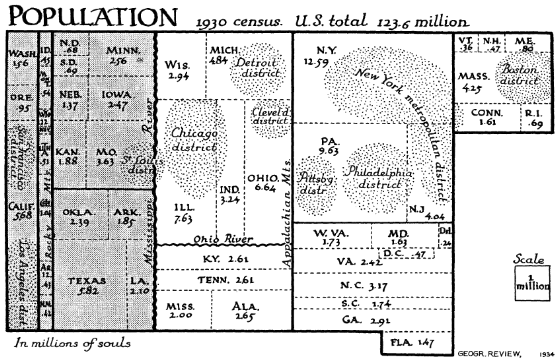
\includegraphics[scale=.8]{introduction/img/cartogram.png}
    \caption{A cartogram by Raisz~\cite{Raisz1934} made in 1934.}
    \label{fig:intro:raisz}
  \end{figure}

\pagebreak[2]
  \begin{wrapfigure}{r}{7cm} %[6]
    \centering
    
\includegraphics[width = 6cm]{introduction/img/areaunivLayout.pdf}
    \caption{Three area-universal layouts.}
    \label{fig:intro:areaunivLayout}
  \end{wrapfigure}
\mypar{Rectangular layout}
  Mathematically, a rectangular cartogram is a  \emph{rectangular layout} (or simply \emph{layout}).
  A layout $\L$ is a partition of an axis-parallel rectangle into a finite set of interior-disjoint axis-parallel rectangles.
  Roughly speaking, we say that two rectangular layouts are \emph{combinatorially equivalent} (or simply \emph{equivalent}) when they have the same adjacencies and these adjacencies are in the same manner, that is horizontal or vertical. We will later, in Section~\ref{s:rel}, define this more thoroughly.
  A rectangular layout is \emph{area-universal} when it has a combinatorially equivalent layout, regardless the area sizes we assign to each rectangle.
  Three area-universal equivalent layouts are given in Figure~\ref{fig:intro:areaunivLayout}.

  The question above then becomes: For which maps can we create area-universal layouts?
  Clearly not those maps that do not have any corresponding layouts with the same adjacencies. However, it will turn out there are more maps without a corresponding area-universal layout.

  \begin{wrapfigure}[8]{r}{7cm}
    \centering
    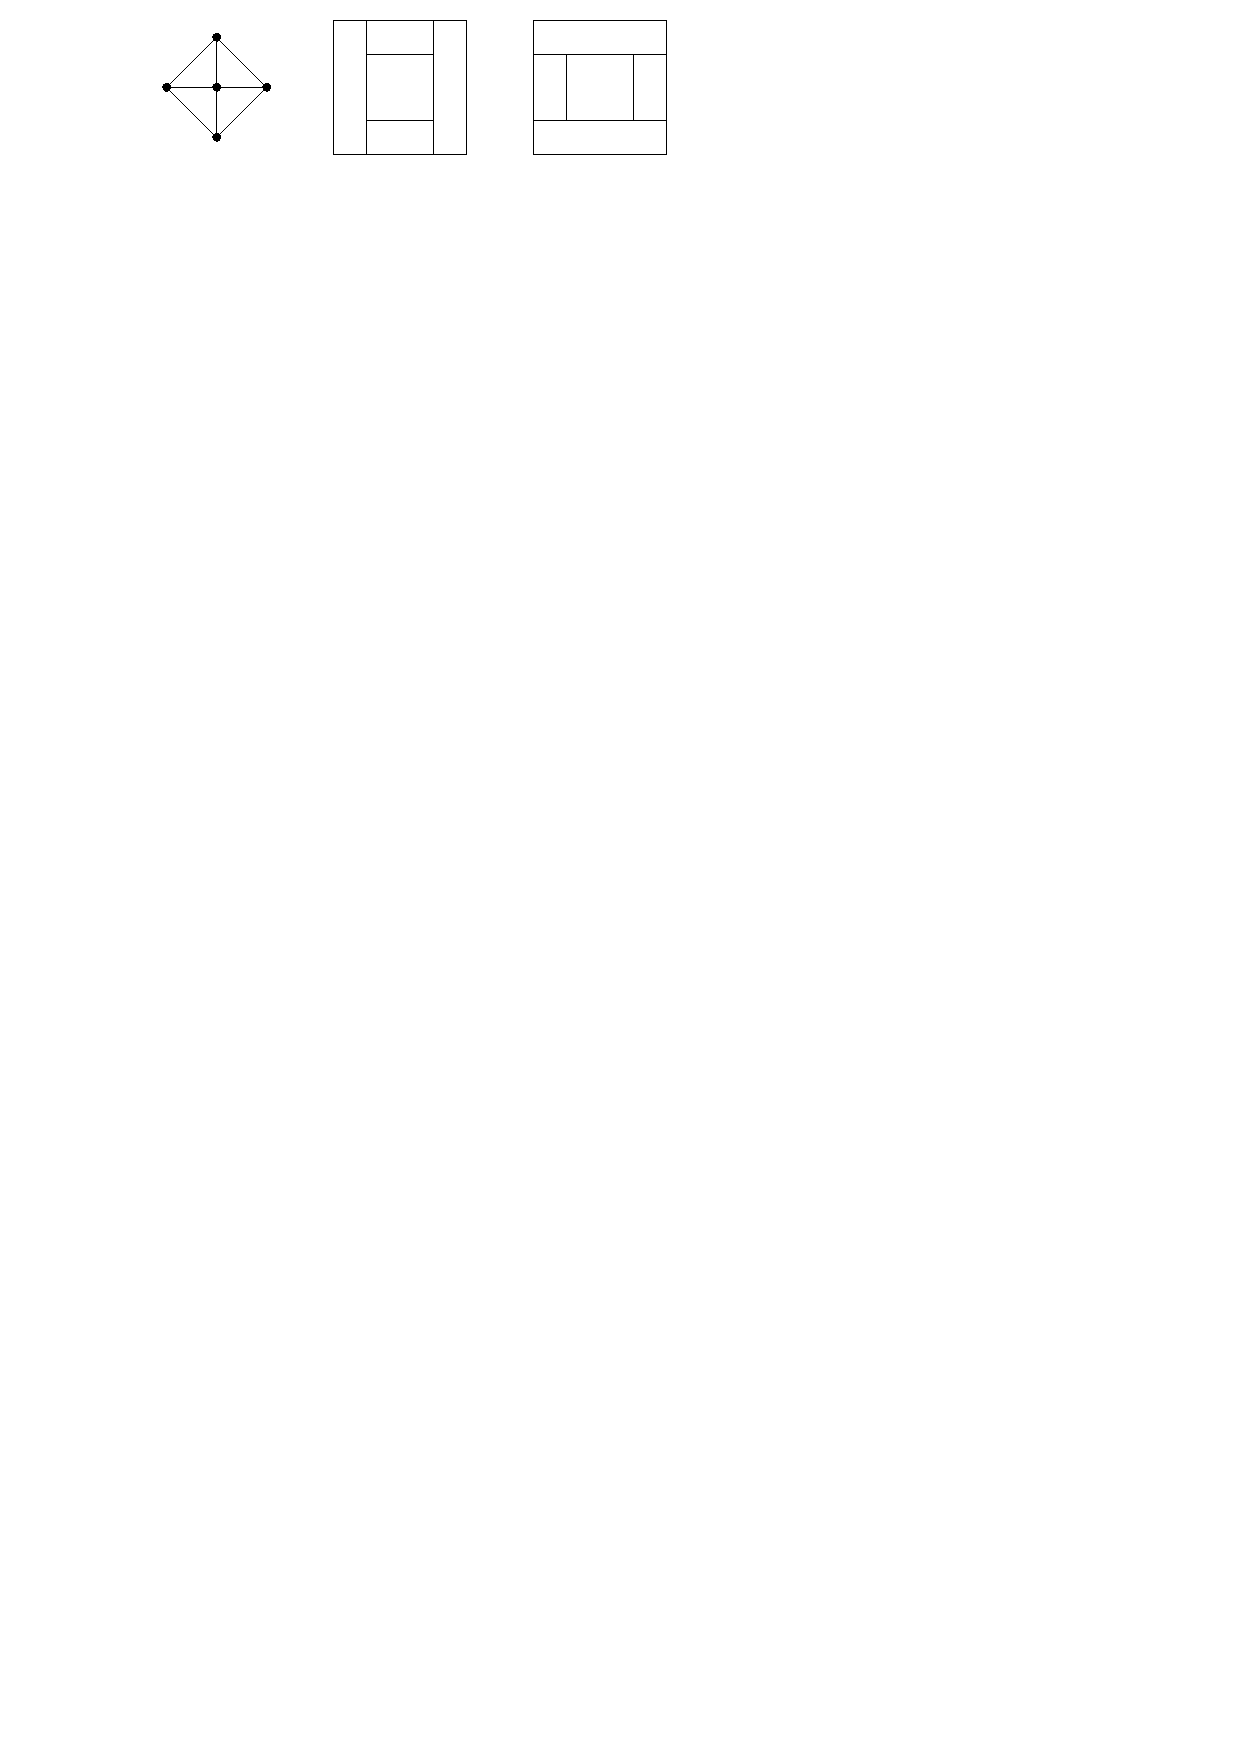
\includegraphics[width=6cm]{introduction/img/nonuniqueRectDual.pdf}
    \caption{A graph with two non-equivalent duals.}
    \label{fig:intro:nonuniqueRectDual}
  \end{wrapfigure}

\mypar{Adjacency graphs}
  We can represent the adjacencies of map regions by an \emph{adjacency graph} $G$ where each region is represented by a vertex and two vertices are connected by an edge exactly when their regions are adjacent.
  Similarly, in the \emph{adjacency graph} $\dualgraph{\L}$ of a rectangular layout $\L$ each rectangle is represented by a vertex and two vertices are connected by an edge exactly when their rectangles are adjacent.
  A layout $\L$ is a \emph{rectangular dual} of a graph $G$ if we have that $G = \dualgraph{\L}$.
  In general, a single graph can have mutiple non-equivalent rectangular duals. An example of this is the graph in Figure~\ref{fig:intro:nonuniqueRectDual}.

  Rinsma found a graph in~\cite{Rinsma1987}, displayed in Figure~\ref{fig:intro:rinsma}, that has no area-universal rectangular duals.
  That is, all rectangular layouts with this graph as adjacency graph are not area-universal.

  \begin{wrapfigure}[14]{r}{5.5cm}  %[13]
    \centering
    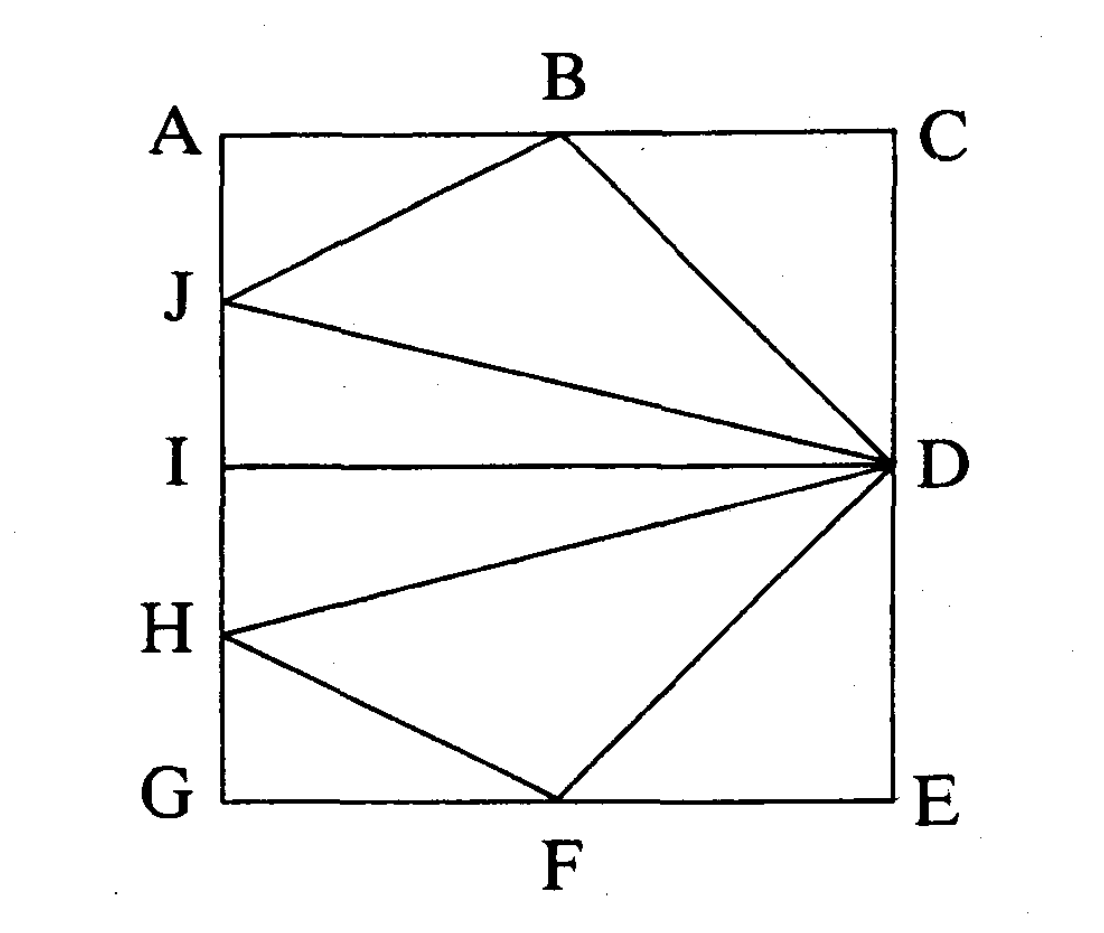
\includegraphics[scale=.16]{introduction/img/rinsma.png}
    \caption{The graph by Rinsma~\cite{Rinsma1987} that is not one-sided.}
    \label{fig:intro:rinsma}
  \end{wrapfigure}

\mypar{One-sided layouts}
  So, unfortunately not all graphs admit area-universal duals.
  We would like to know which graphs do.
  Before we can state this we need to define one-sided layouts.
  Note that the interior of a rectangular layout contains vertical and horizontal line segments.
  Any line segment that can not extend any farther on either side is a \emph{maximal segment}.
  A rectangular layout is \emph{one-sided} if every maximal segment has only one rectangle on one of its sides.
  The layouts in Figure~\ref{fig:intro:areaunivLayout} and  \ref{fig:intro:nonuniqueRectDual} are all one-sided.

  In~\cite{Eppstein2012} Eppstein et al. show that rectangular layouts are area-universal exactly when they are one-sided.
  So, Rinsma's result also implies that not every adjacency graph of a map can be represented by a one-sided layout.


\mypar{$\mathbf{k}$-sided layouts}
  \begin{figure}[t]
    \quad
    \begin{subfigure}[b]{0.45 \textwidth}
      \centering
      
\includegraphics[width=\textwidth]{introduction/img/2sidedBefore.pdf}
      \caption{Before resizing $a$}
      \label{fig:intro:2sidedBefore}
    \end{subfigure}
    \hfill
    \begin{subfigure}[b]{0.45 \textwidth}
      \centering
      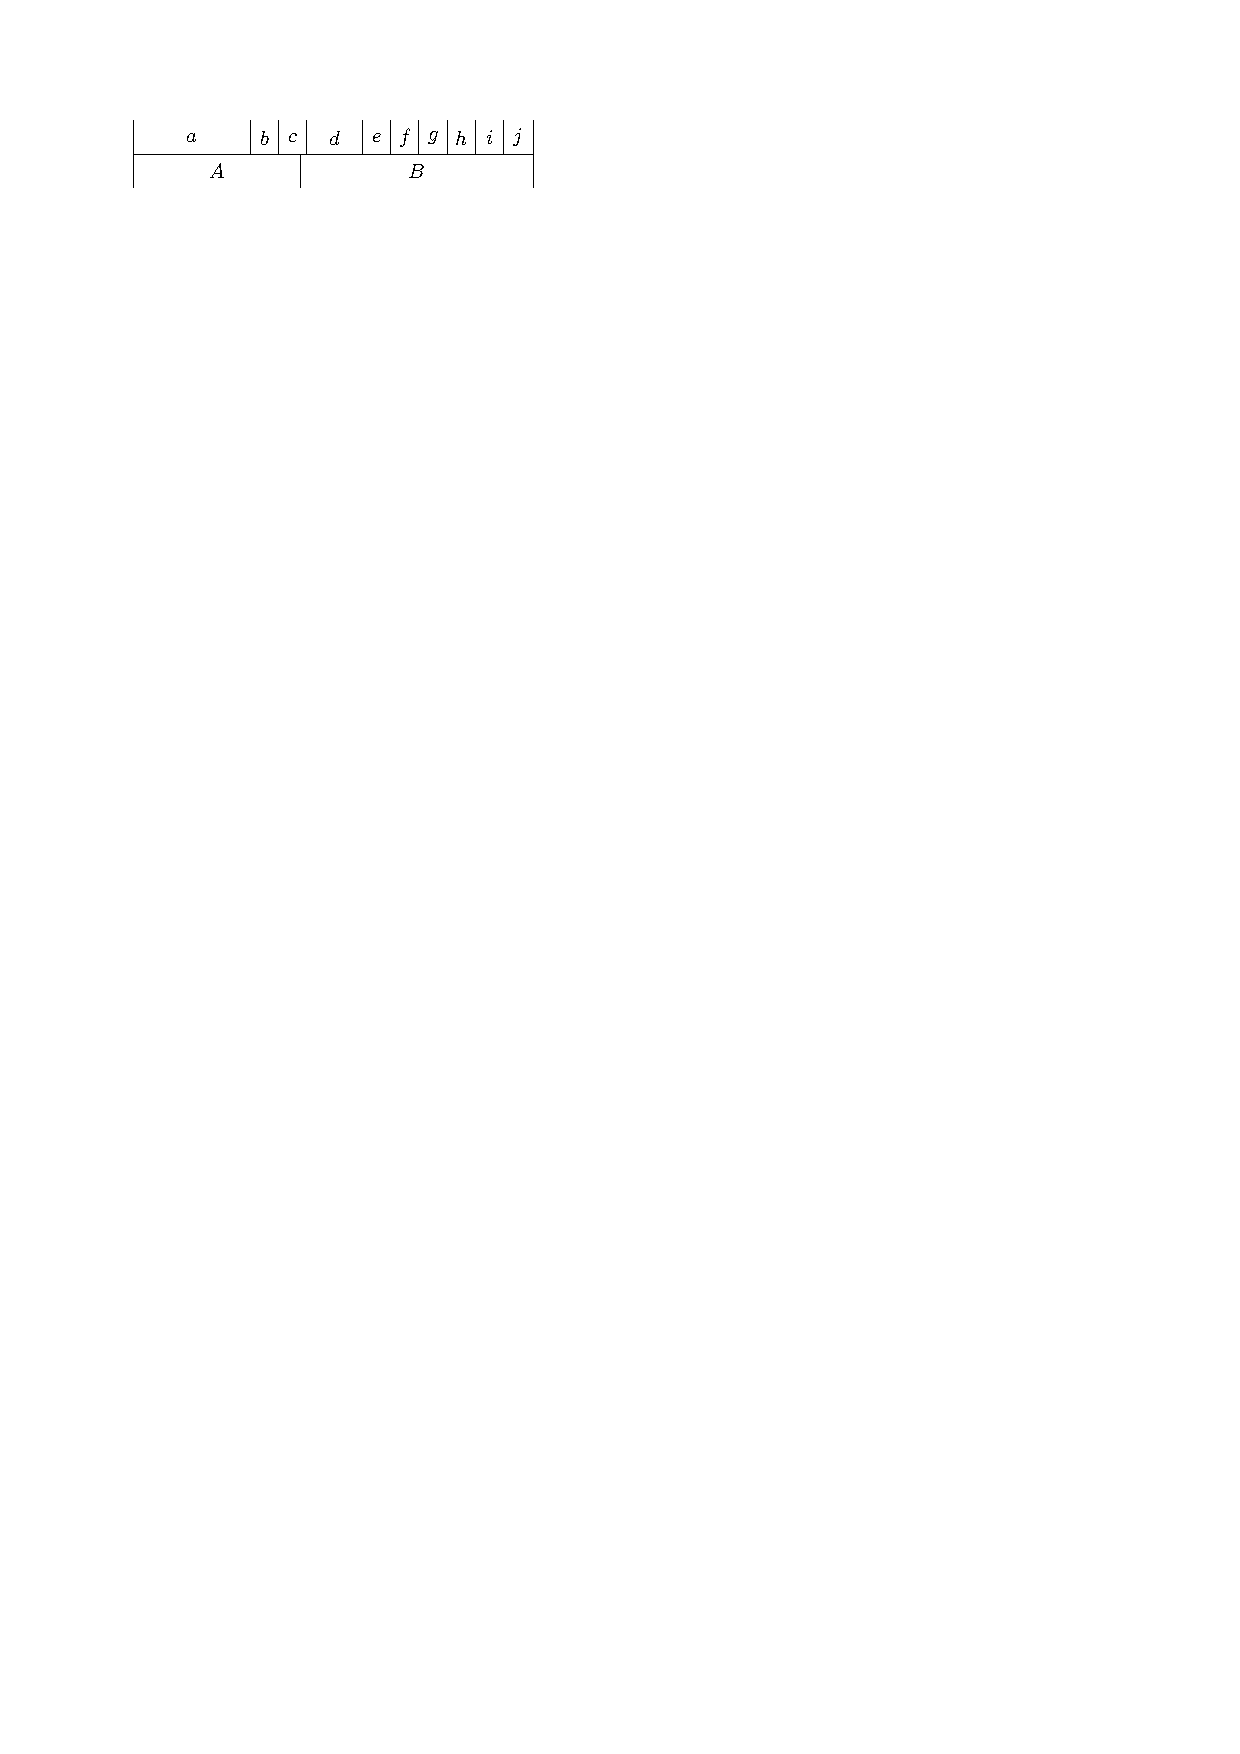
\includegraphics[width=\textwidth]{introduction/img/2sidedAfter.pdf}
      \caption{After resizing $a$}
      \label{fig:intro:2sidedAfter}
    \end{subfigure}
    \caption{A 2-sided segment}
    \label{fig:intor:2sided}
    \quad

    \quad
    \begin{subfigure}[b]{0.45 \textwidth}
      \centering
      
\includegraphics[width=\textwidth]{introduction/img/10sidedBefore.pdf}
      \caption{Before resizing $a$}
      \label{fig:intro:10sidedBefore}
    \end{subfigure}
    \hfill
    \begin{subfigure}[b]{0.45 \textwidth}
      \centering
      
\includegraphics[width=\textwidth]{introduction/img/10sidedAfter.pdf}
      \caption{After resizing $a$}
      \label{fig:intro:10sidedAfter}
    \end{subfigure}
    \quad
    \caption{A 10-sided segment}
    \label{fig:intro:10sided}
  \end{figure}
  Let us consider those graphs that do not admit any one-sided, and thus area-universal, dual as rectangular dual.
  Since any dual for such a graph is not area-universal, it is inevitable that adjacencies between rectangles in this dual change when we resize them.
  For these graphs we want to find layouts that have the least number of adjacency changes when area sizes change.
  This is beneficial for, for example, applications displaying cartograms on a continuous timescale.
  Since every time the adjacencies of the layout change, we have to compute a different rectangular layout with the right adjacencies, providing the user a rougher viewing experience.

  We call a layout \emph{$k$-sided} if $k$ is the smallest integer such that every maximal segment has at most $k$ rectangles on one of its sides. This is a direct generalization of one-sidedness.
  This generalization is useful because, when changing the areas of rectangles in a $k$-sided layout fewer adjacencies change, in general, if $k$ is small then if $k$ is large.

  We illustrate this by comparing a typical $2$-sided and a typical $10$-sided segment.
  Let us first consider the $2$-sided segment in Figure~\ref{fig:intro:2sidedBefore}, if the size of $a$ doubles only two adjacencies change, namely $dA$ disappears and $cB$ appears, as can been seen in Figure~\ref{fig:intro:2sidedAfter}.
  While for a typical $10$-sided segment doubling the size of $a$ leads to $15$ changed adjacencies, namely $aC$ $aD$ $ bB$ $ bC$ $ bD$ $ bE$ $ cC$ $ cD$ $ cE$ $ cF$ $ dE$ $ dG$ $ eF$ $ eH$ $ fG$, as can been seen in Figure~\ref{fig:intro:10sided}.
  Hence we would like to find $k$-sided layouts for all graphs with $k$ as small as possible.


\mypar{Counterexample}
  In this thesis we provide two results on $k$-sidedness. The first result is the existence of a family of graphs $G_k$ that, for any constant $k \in \N$, has members that are not $k$-sided (Theorem \ref{fix:th:family}). The family of graphs in this result is characterized by the occurrence of nested separating $4$-cycles.
  A \emph{$4$-cycle} is a cycle of length $4$.
  Such a cycle is separating if there are vertices in both its interior and exterior.
  Separating $4$-cycles are \emph{nested} if one is contained in the other, but some of their vertices overlap. These different types of $4$-cycles are demonstrated in Figure~\ref{fig:intro:4cycle}.

  \begin{wrapfigure}{r}{7cm}
      \centering
      \begin{subfigure}[t]{2cm}
          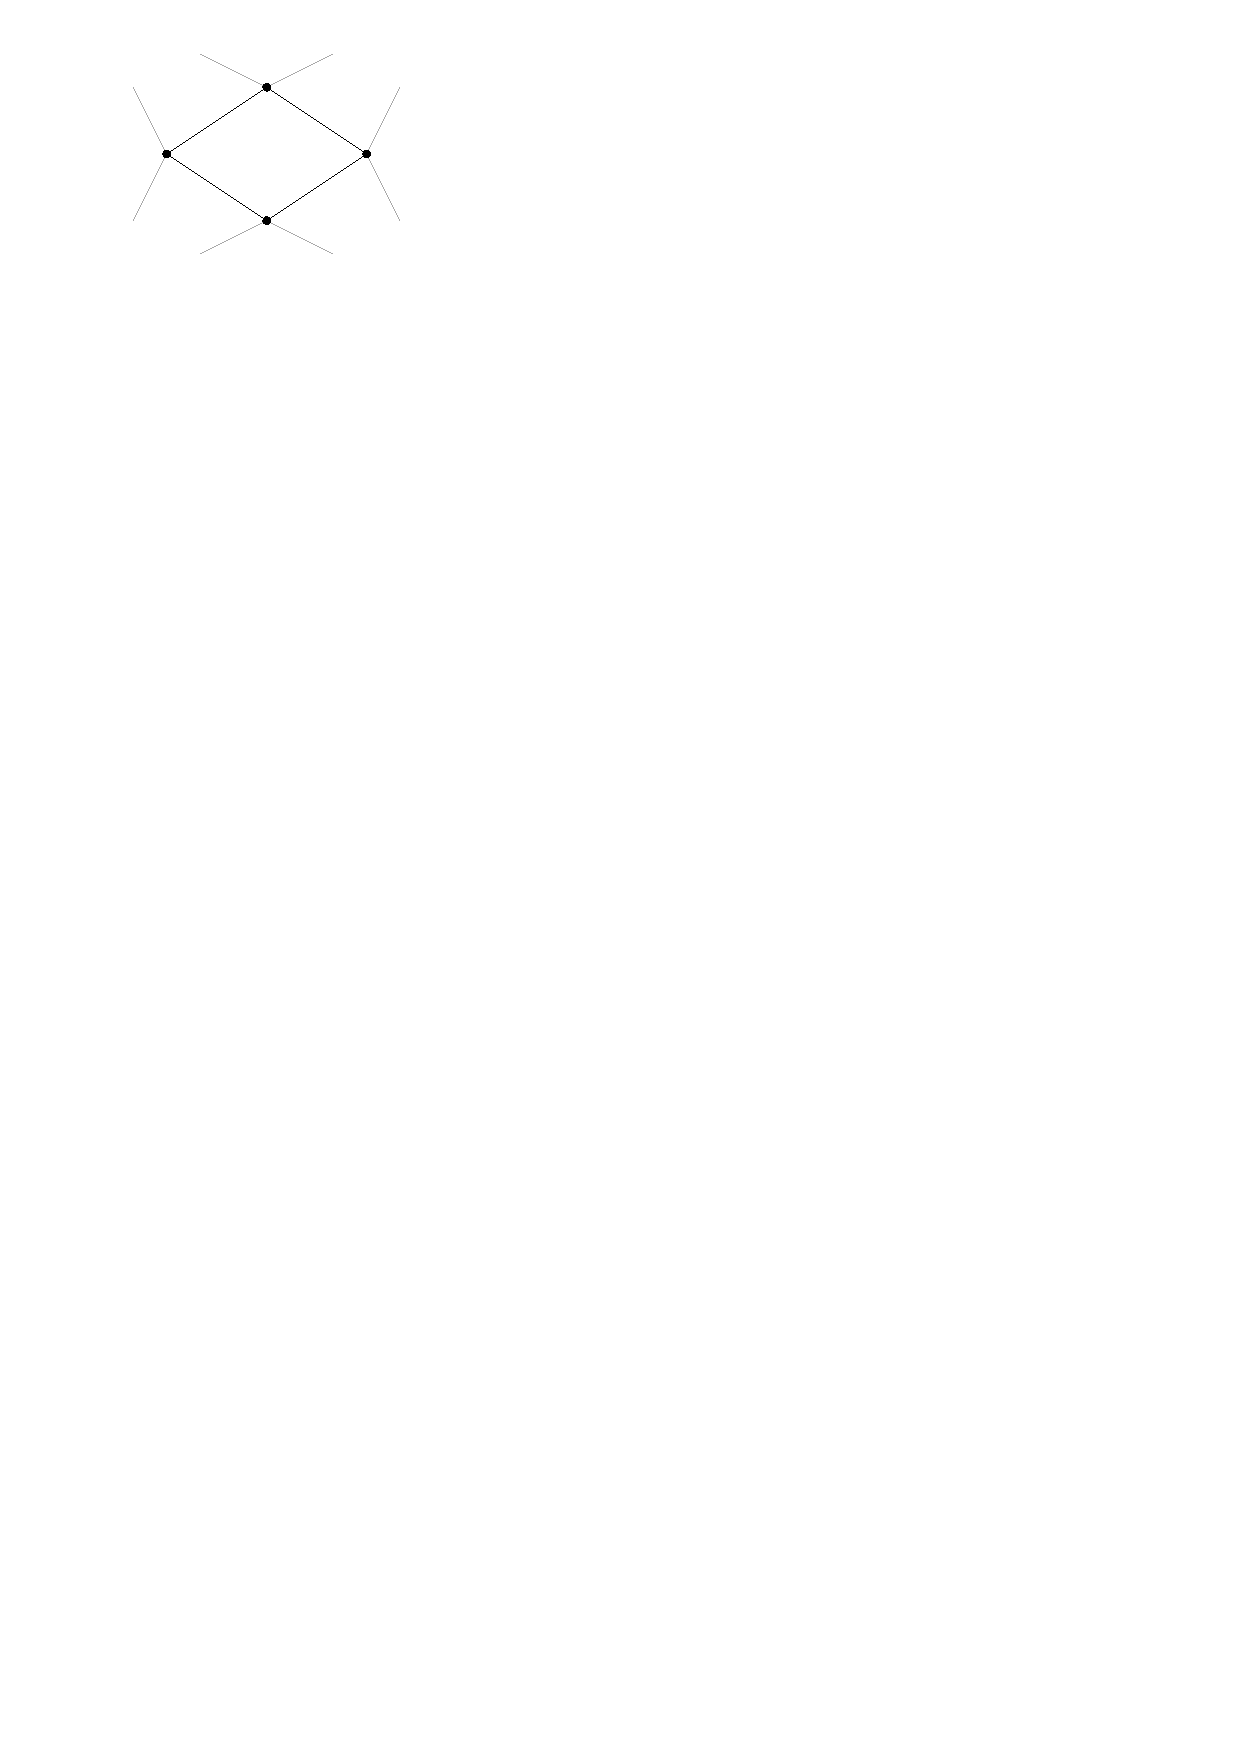
\includegraphics[width = \textwidth]{introduction/img/4cycle.pdf}
          \caption{A $4$-cycle.}
      \end{subfigure}
      ~
      \begin{subfigure}[t]{2cm}
          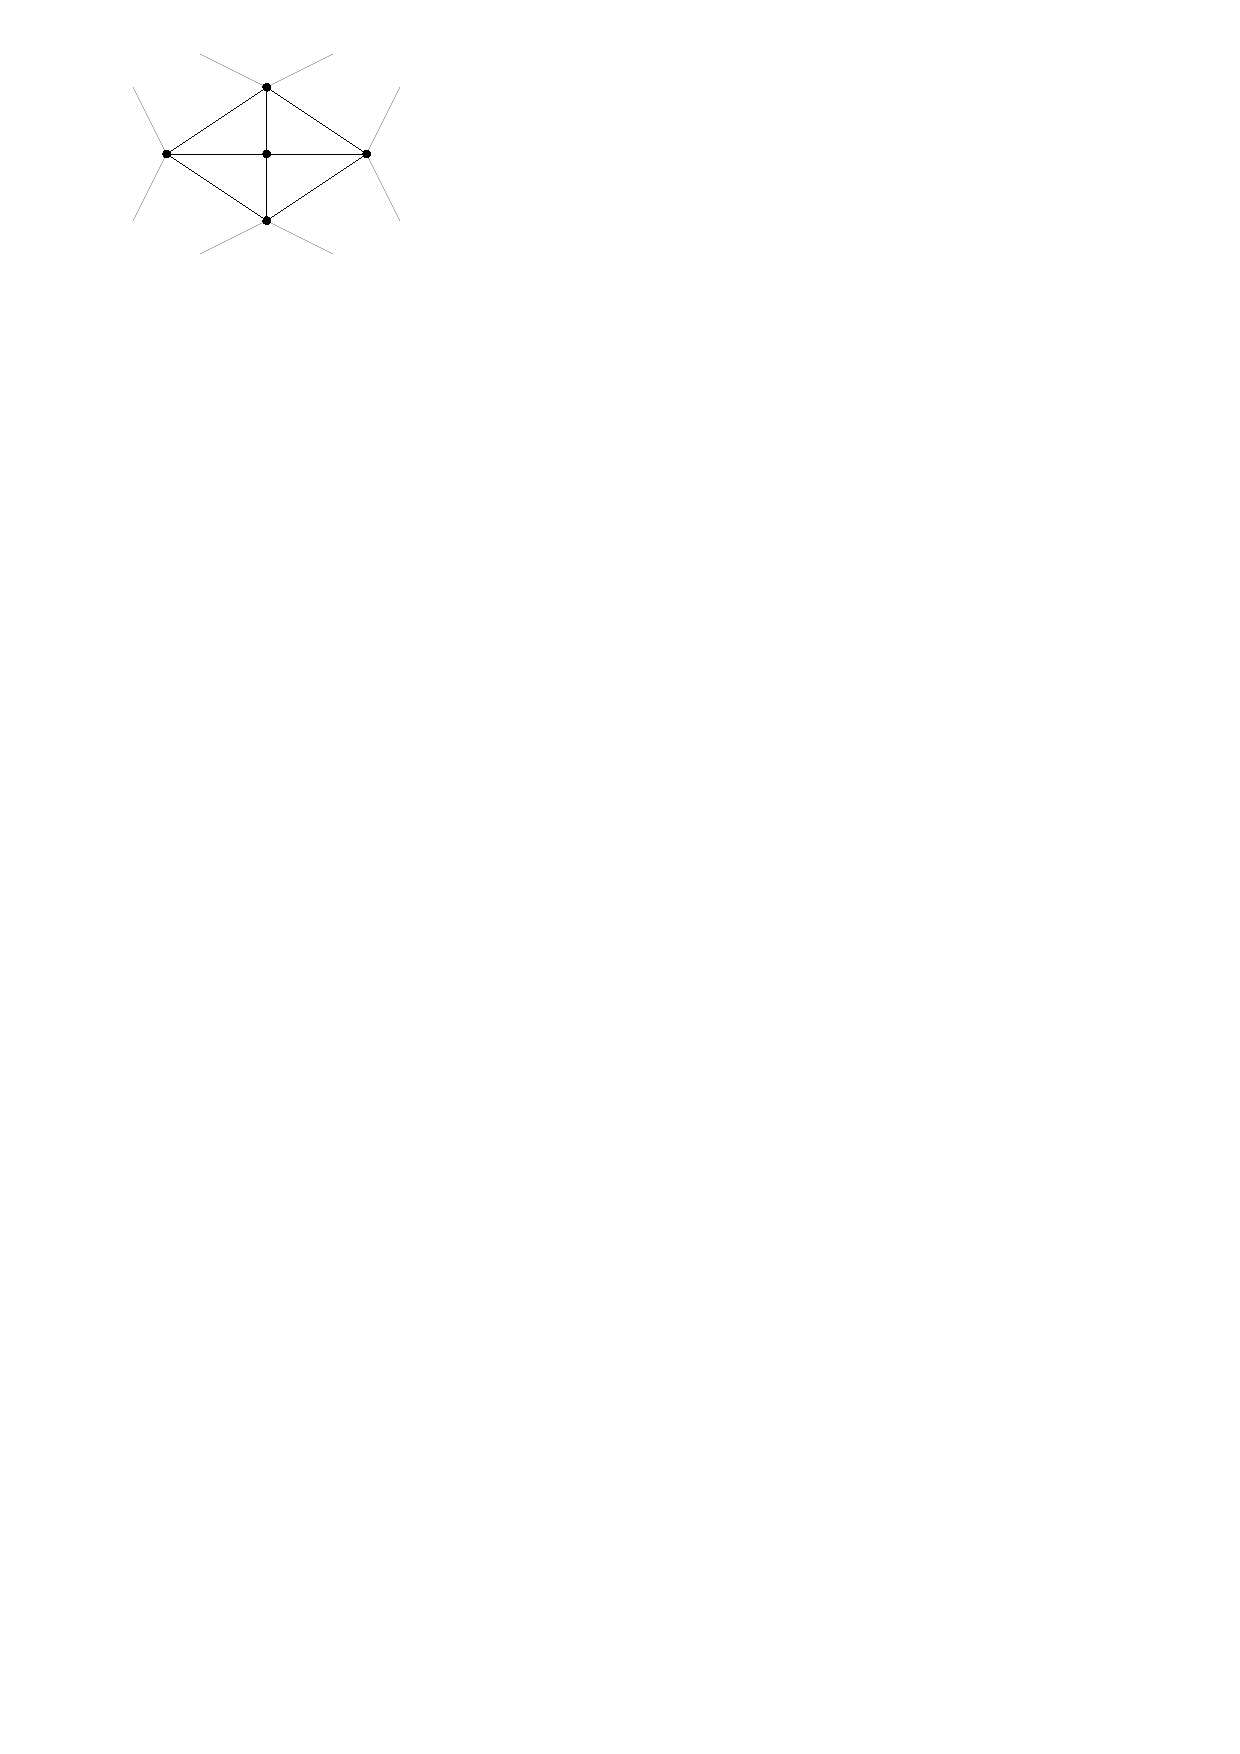
\includegraphics[width = \textwidth]{introduction/img/sep4cycle.pdf}
          \caption{A separating $4$-cycle.}
      \end{subfigure}
      ~
      \begin{subfigure}[t]{2cm}
          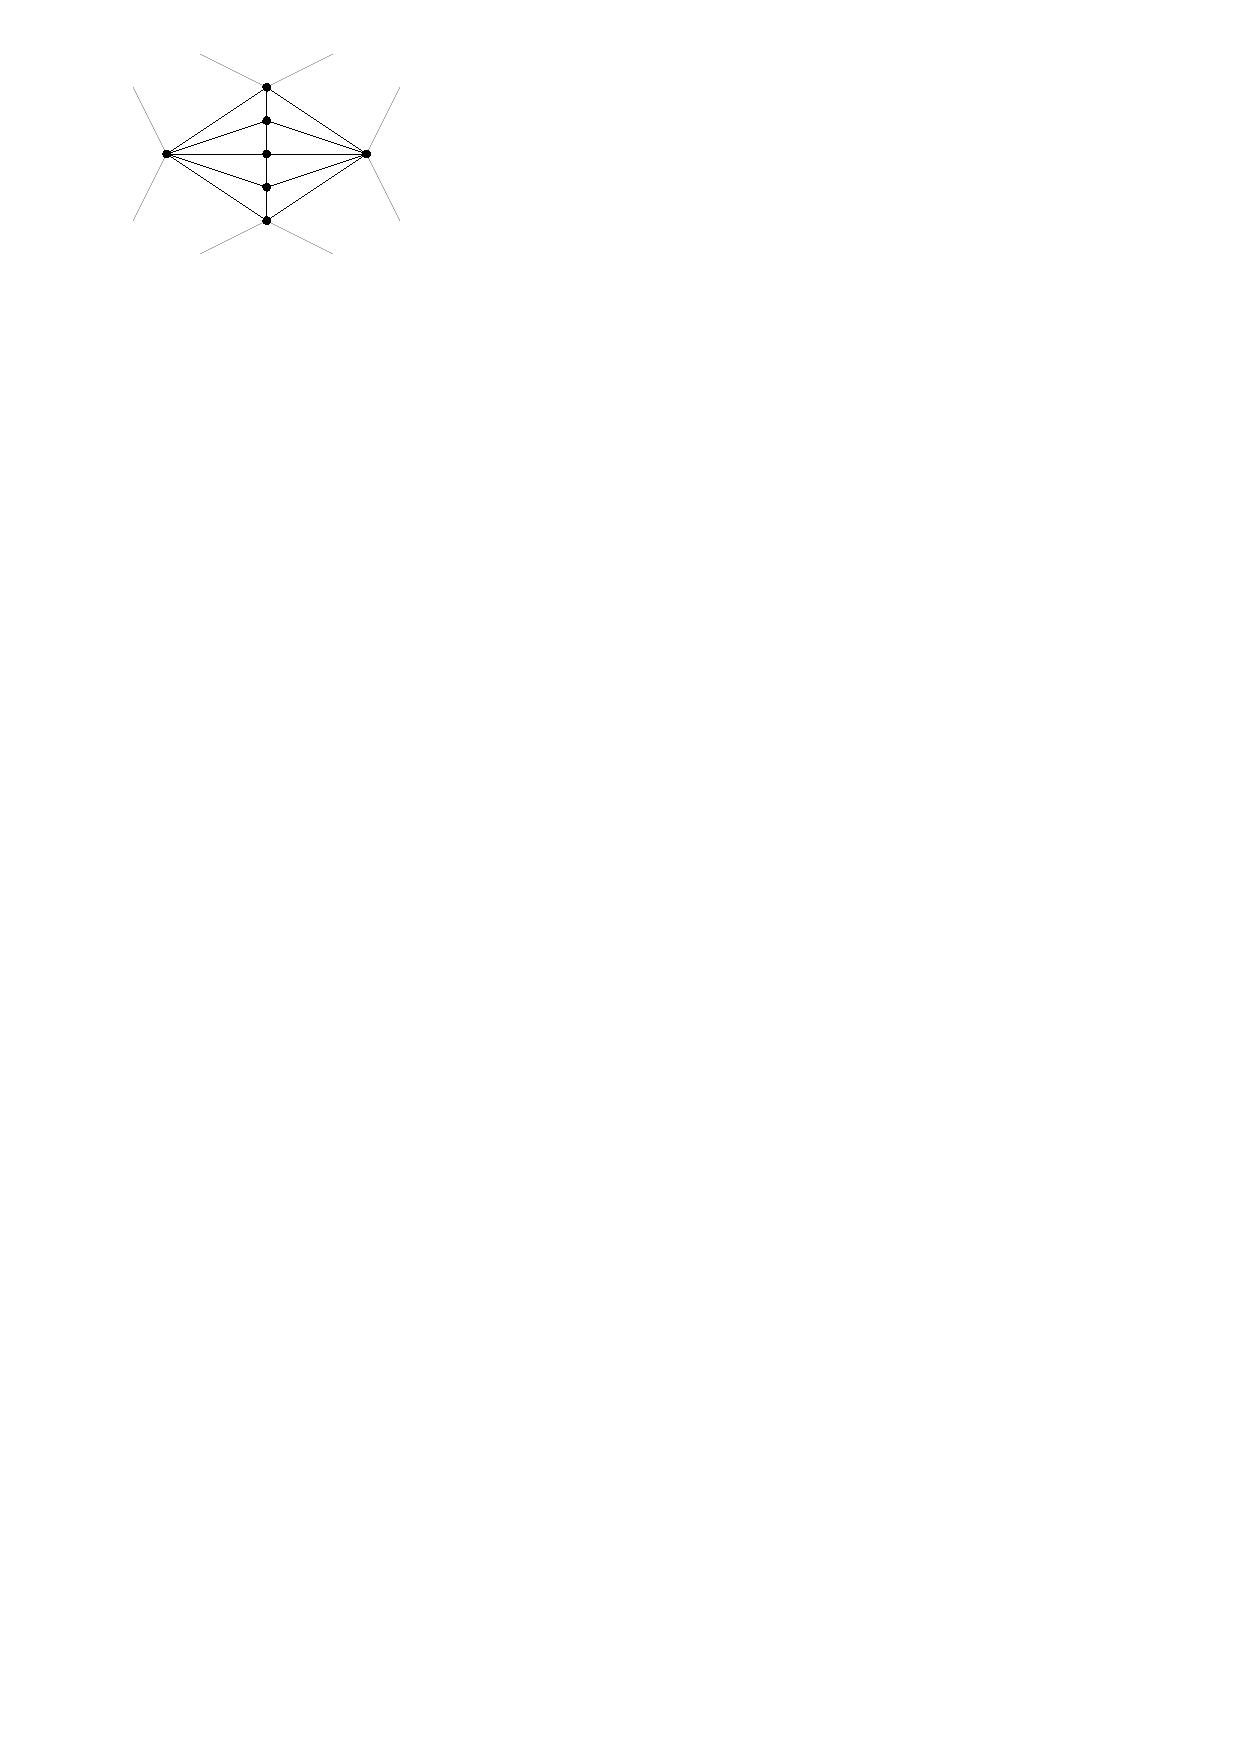
\includegraphics[width =\textwidth]{introduction/img/nest4cycle.pdf}
          \caption{A nested separating 4-cycle.}
      \end{subfigure}
    \caption{}
    \label{fig:intro:4cycle}
  \end{wrapfigure}


  Separating $4$-cycles in general are difficult to treat when trying to create a $k$-sided layout.
  But examples found during our research seem to indicate that, in particular, nested $4$-cycles are the most difficult to treat.
  Finding $k$-sided rectangular duals is not the only problem that has difficulty with separating $4$-cycles.

  Yeap and Sarrafzadeh~\cite{Yeap1995} investigated the problem of finding a \emph{sliceable} dual for a graph. A rectangular layout is sliceable when it is either a single rectangle or when it has a single maximal segment which splits the layout into two sliceable layouts.
  Yeap and Sarrafzadeh were able to show that all graphs without a separating $4$-cycle have a sliceable rectangular dual.
  They were unable to gain traction on graphs with a separating $4$-cycle (in their words this is a complex cycle of length~4).

  \begin{wrapfigure}[12]{r}{7cm}
    \centering
      \begin{subfigure}[t]{3cm}
        \centering
        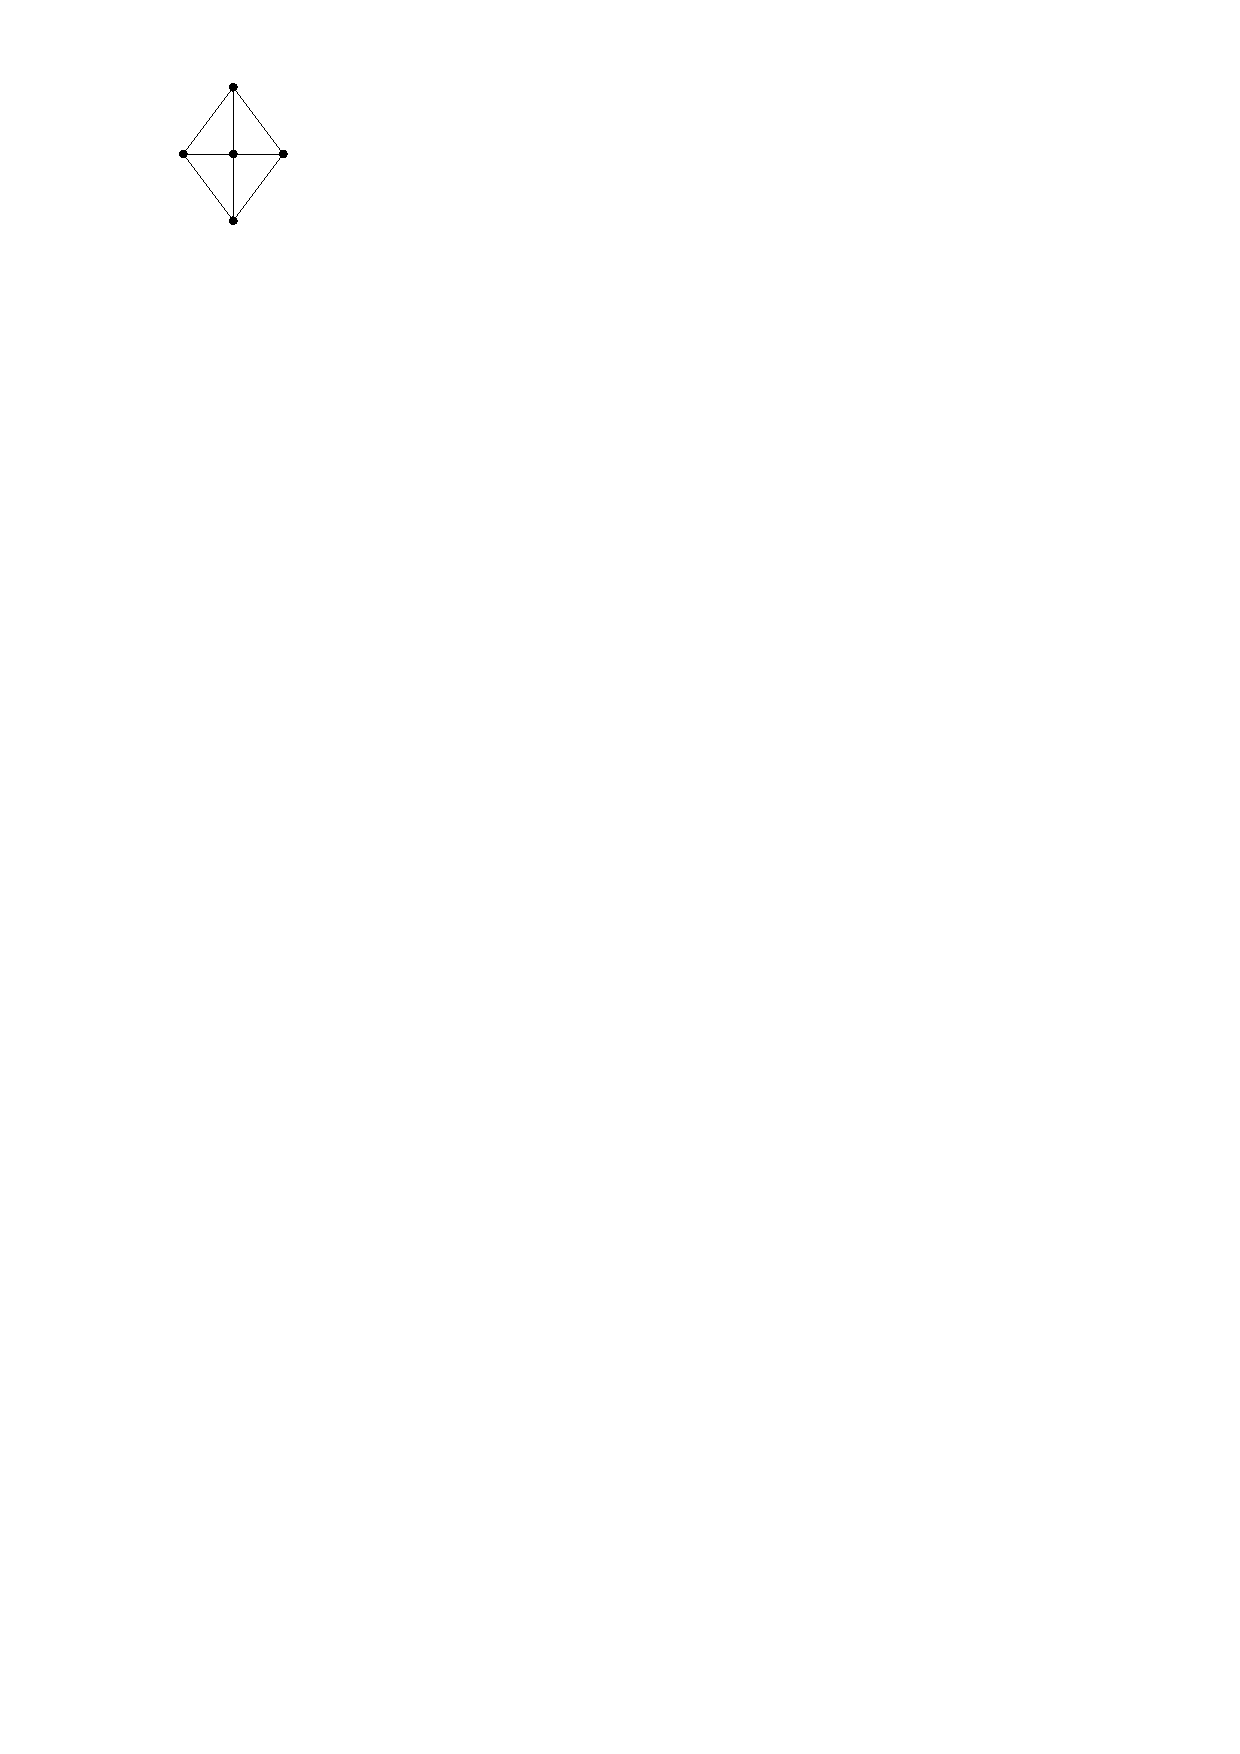
\includegraphics[scale=1]{introduction/img/areaunivGraph.pdf}
        \caption{Graph with separating 4-cycle.}
      \end{subfigure}
      ~
      \begin{subfigure}[t]{3cm}
        \centering
        
\includegraphics[scale=1]{introduction/img/areaunivDual.pdf}
        \caption{Corresponding area-universal dual.}
      \end{subfigure}
    \caption{}
    \label{fig:intro:areauniv}
  \end{wrapfigure}

  Nevertheless, not all problems are intractable on graphs with a separating $4$-cycle.
  The problem of finding an area-universal rectangular dual of a graph, already mentioned above, was investigated by Eppstein et al.  in~\cite{Eppstein2012}.
  They managed to find such a rectangular dual, when it exists, for any graph $G$.
  This result does affect graphs containing separating $4$-cycles since there are such graphs that admit area-universal duals, as can been seen in Figure~\ref{fig:intro:areauniv}.


  \begin{wrapfigure}[]{r}{8cm}
    \centering
      \begin{subfigure}[t]{1.3cm}
        \centering
        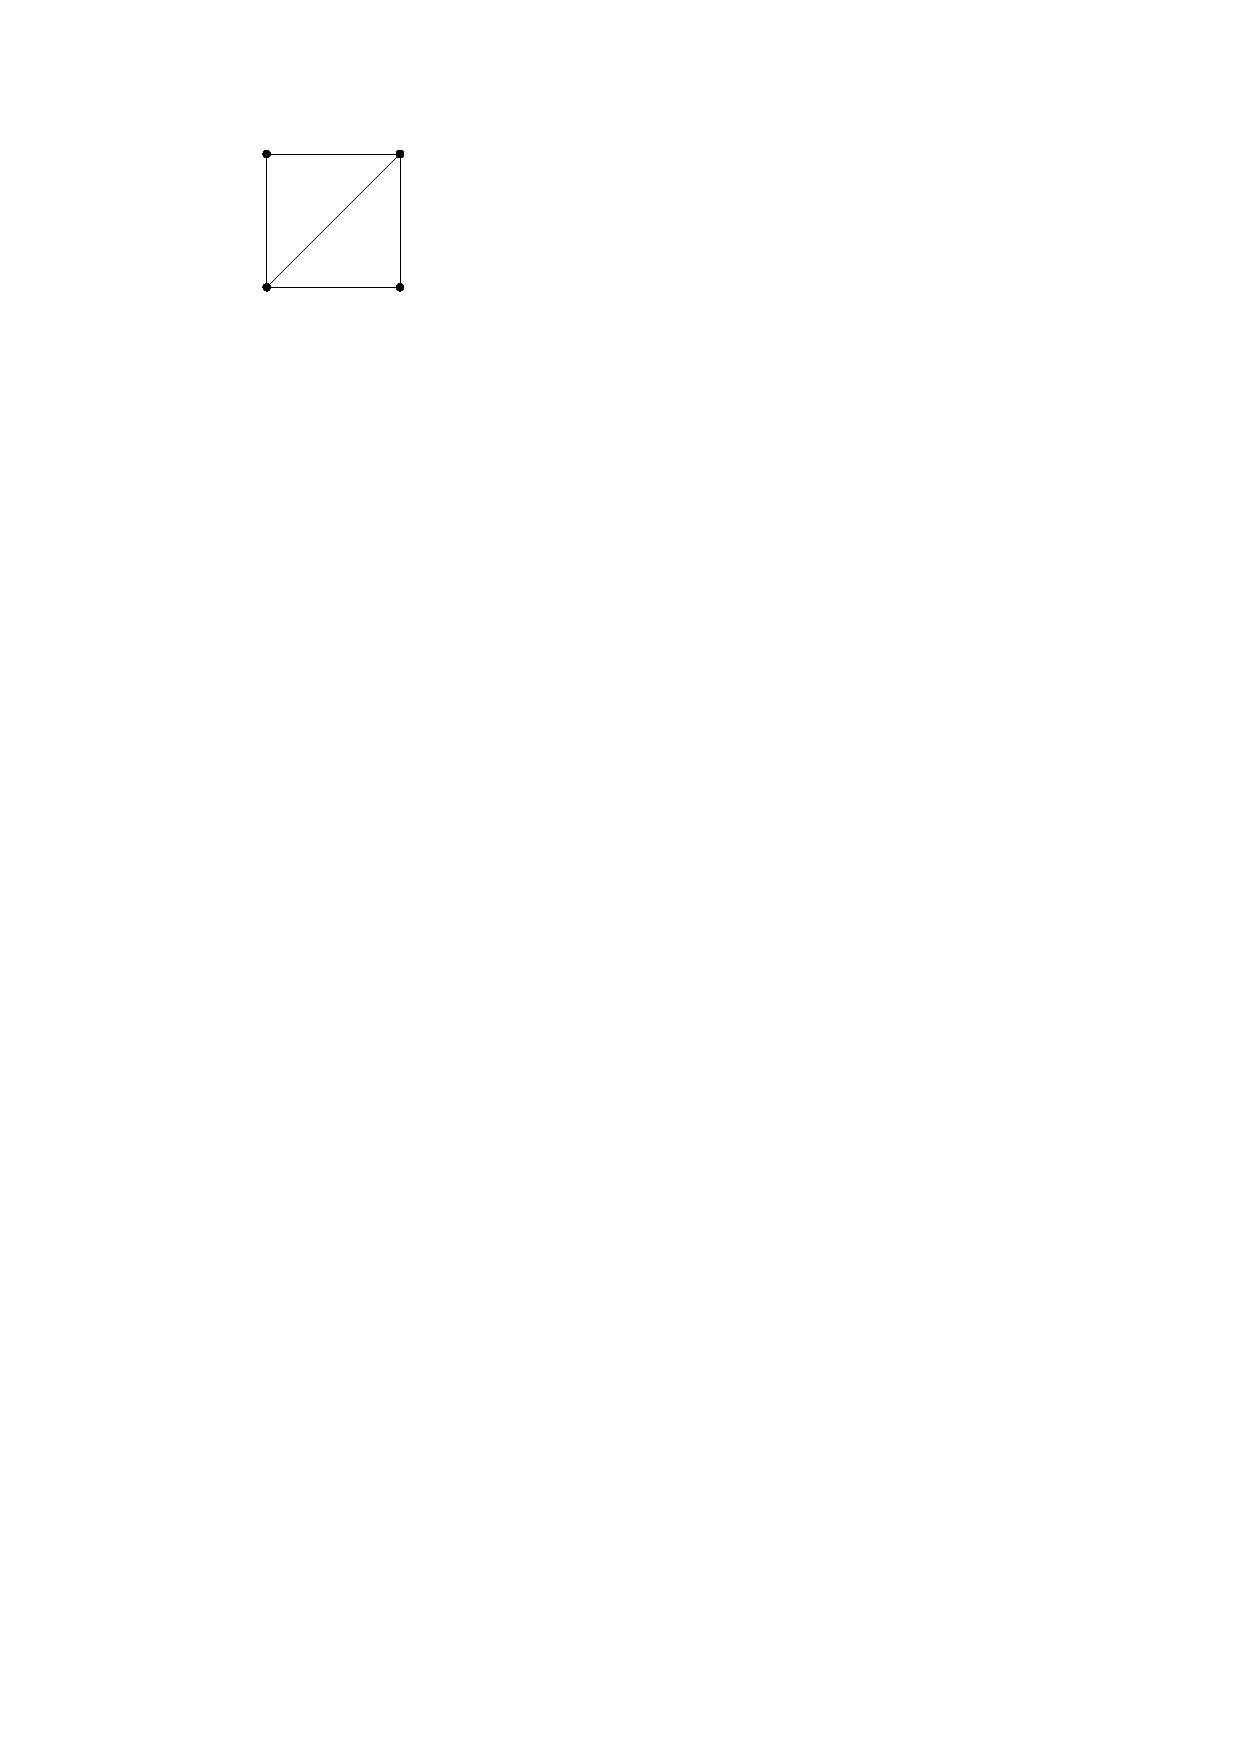
\includegraphics[scale=.3]{introduction/img/caGraph.pdf}
        \caption{A graph $G$.}
      \end{subfigure}~
      \begin{subfigure}[t]{3cm}
        \centering
        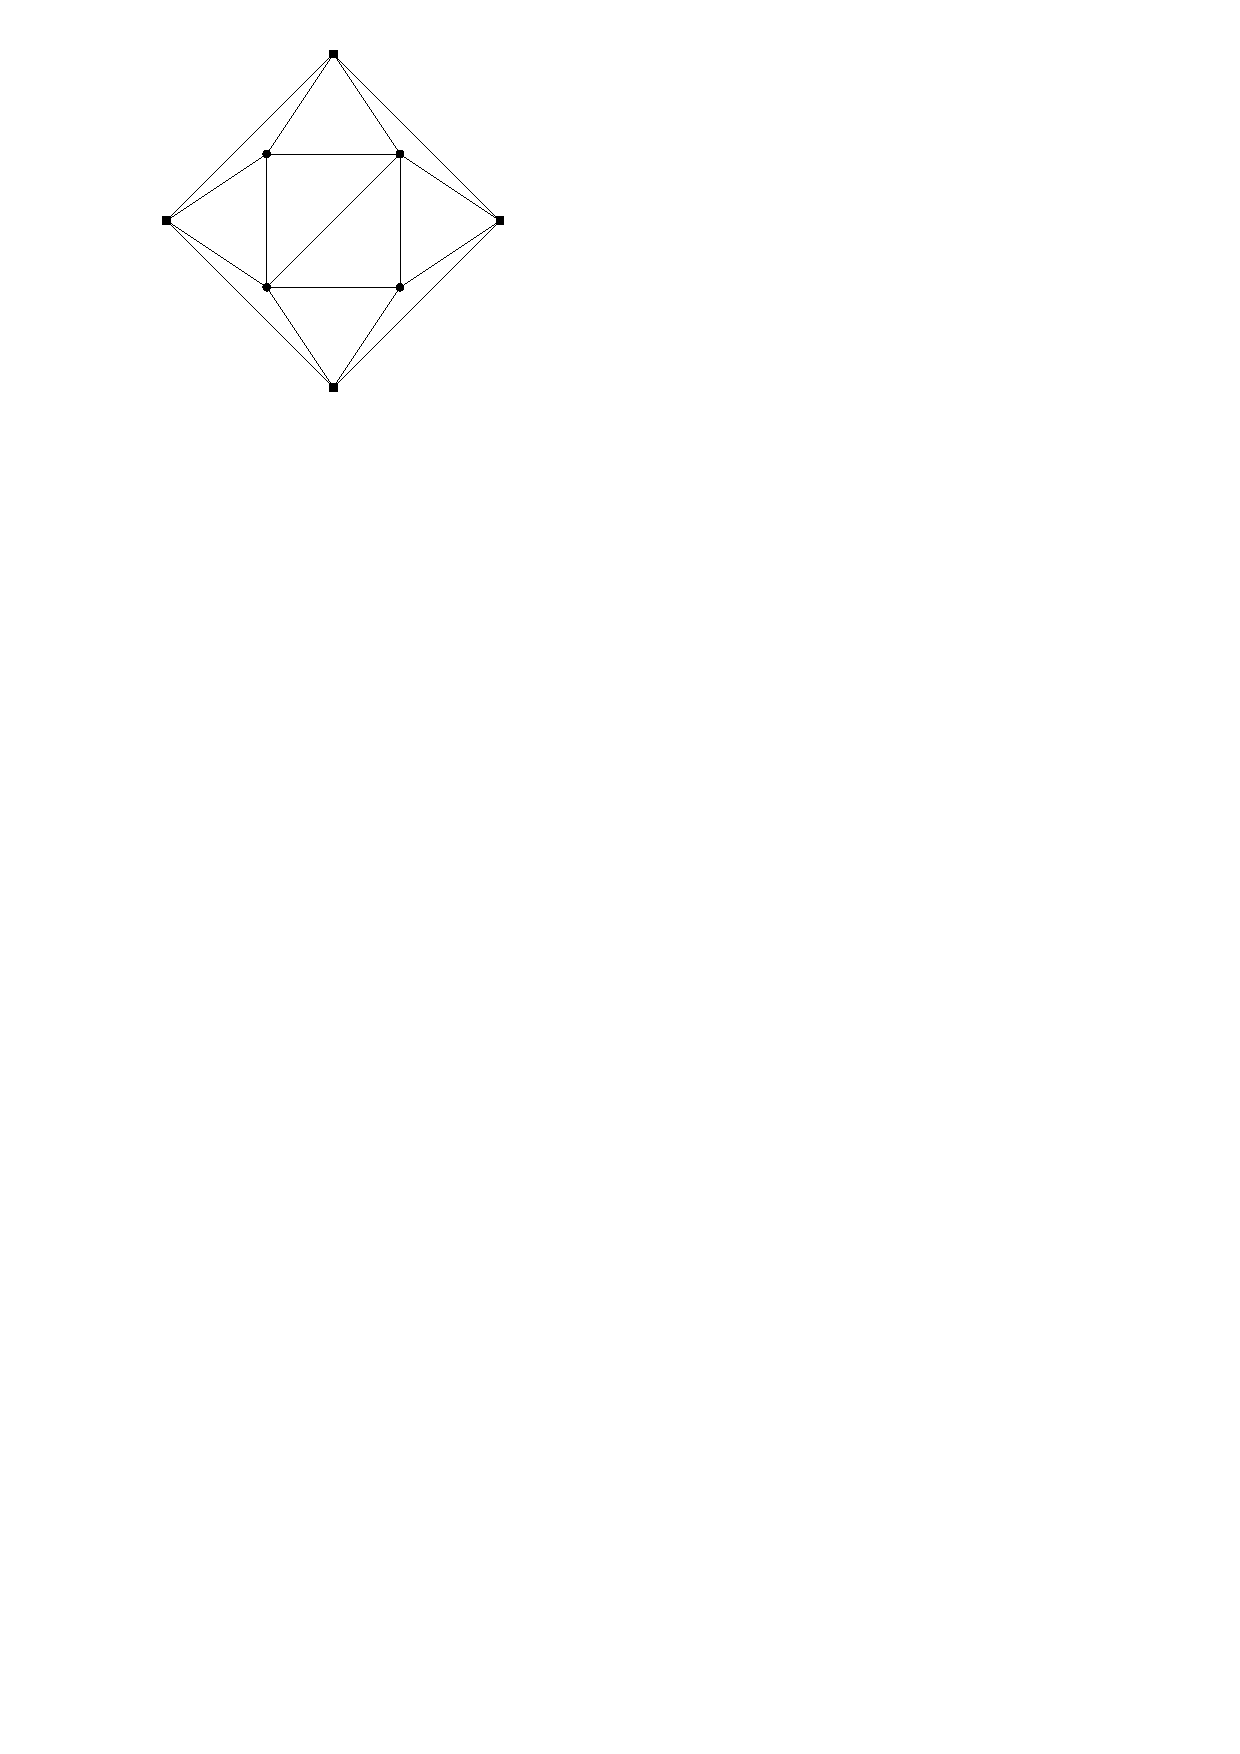
\includegraphics[scale=.3]{introduction/img/caCa.pdf}
        \caption{A corner assignment of $G$.}
      \end{subfigure}~
      \begin{subfigure}[t]{3cm}
        \centering
        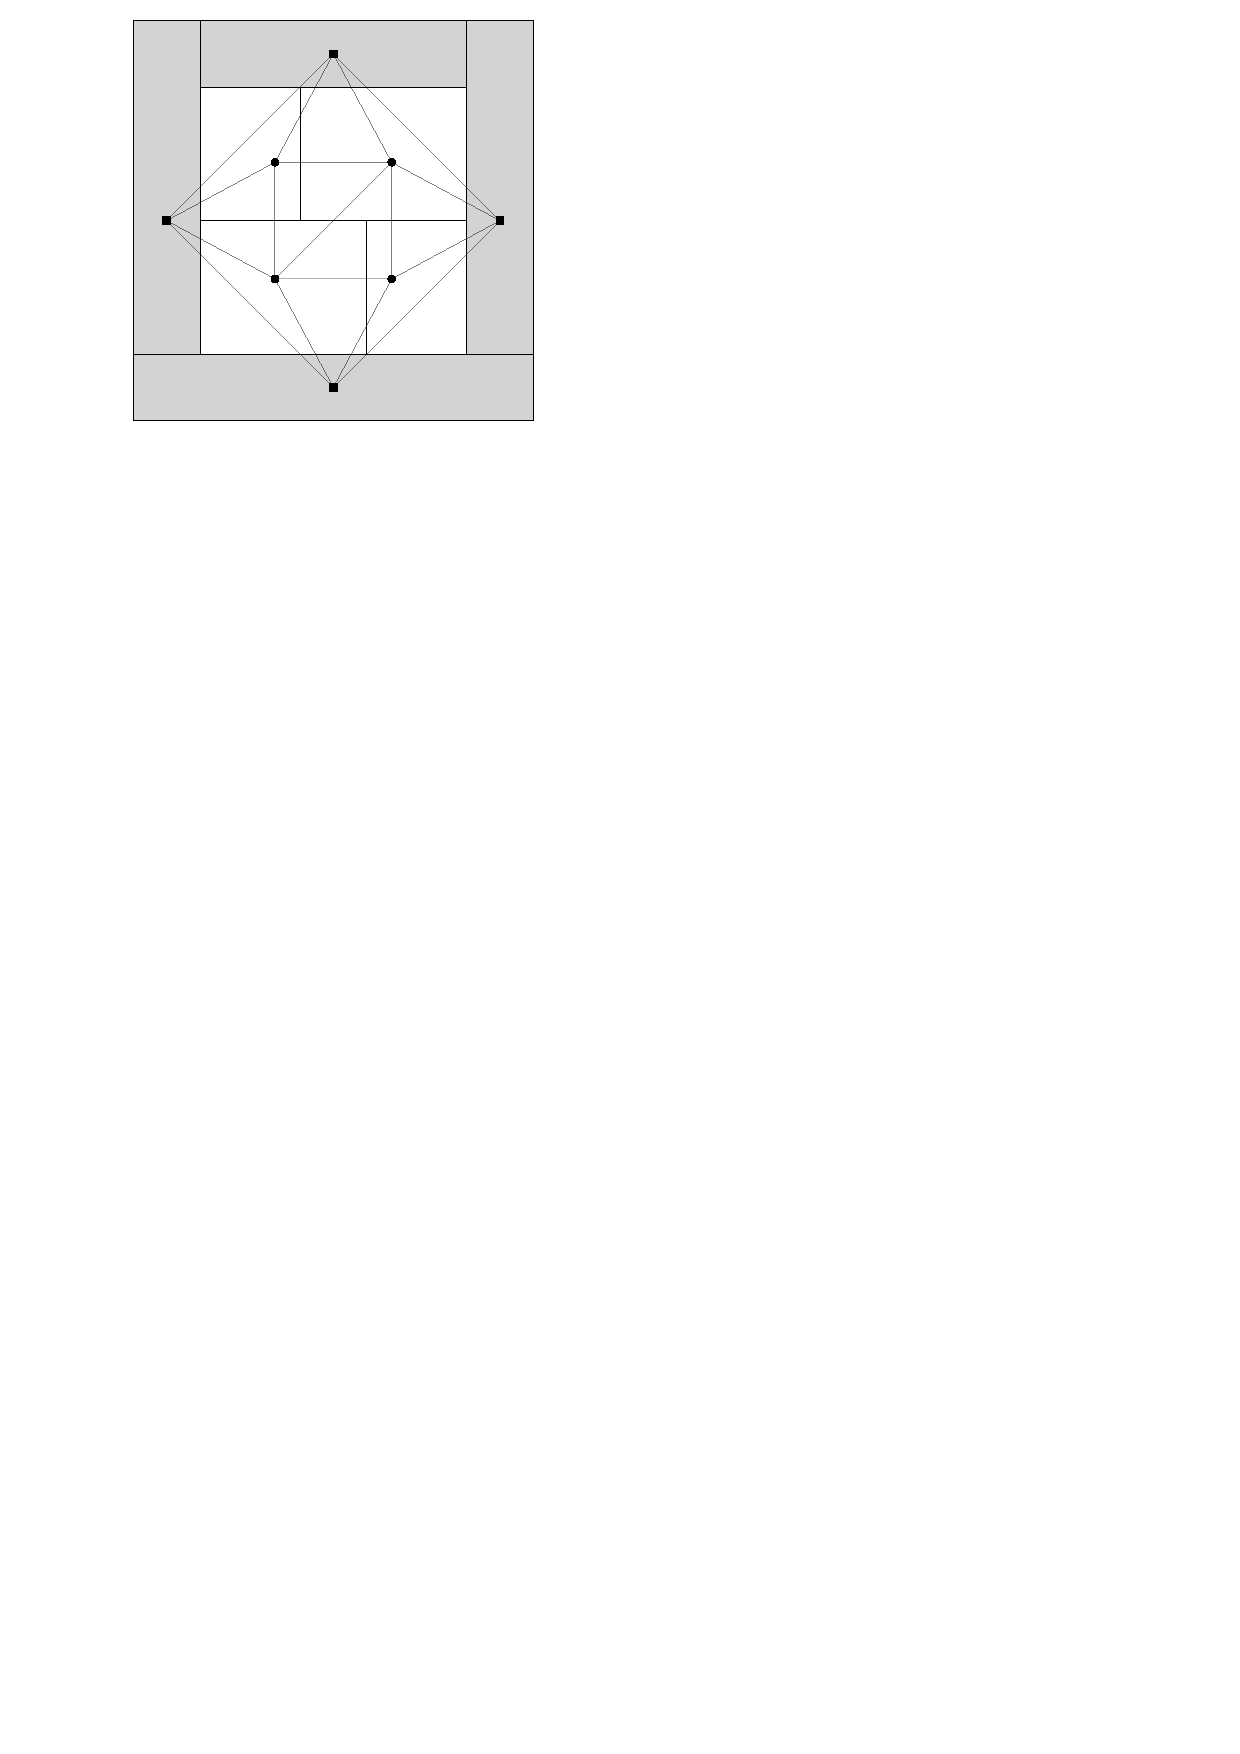
\includegraphics[scale=.3]{introduction/img/caDual.pdf}
        \caption{A rectangular dual corresponding to this corner assignment.}
      \end{subfigure}
    \caption{}
    \label{fig:intro:cornerAssign}
  \end{wrapfigure}

\mypar{Corner assignments}
  Before we can state the second result of this thesis, we first introduce the concept of corner assignments.
  A corner assignment $\ext G$ of a graph $G$ is an augmentation of $G$ with $4$ external vertices, which we call its \emph{poles}, with the following three properties (i) every interior face has degree $3$, (ii) the exterior face has degree $4$ and (iii) $\ext G$ has no separating triangles.
  A corner assignment fixes which rectangles are in the corners of the rectangular dual $\L$, namely those adjacent to two poles, which explains the terminology. In Figure~\ref{fig:intro:cornerAssign} we see a graph, a possible corner assignment of this graph, and a possible rectangular dual (in this case, up to equivalence, the only possible dual) of this corner assignment.

\mypar{Existence of rectangular duals}
  Now we have formulated corner assignments we can also state which graphs admit rectangular duals.
  A graph admits a rectangular dual if and only if it admits a corner assignment.
  This was shown independently by Kozminski and Kinnen \cite{Kozminski1984} and Ungar \cite{Ungar1953}.

\mypar{Algorithm}
  After finding the counterexample, we focused our efforts on obtaining an algorithm that would provide a $k$-sided layout for corner assignments without a separating $4$-cycle, for some constant $k \in \N$.
  Unfortunately, we fell short of this goal and only found an algorithm that provides a $d-1$-sided layout, where $d$ is the maximal degree of the vertices of $G$ in the corner assignment $\ext G$ (Theorem \ref{th:dsided}).

  \begin{wrapfigure}[14]{r}{4.6cm} %[13]
    \centering
    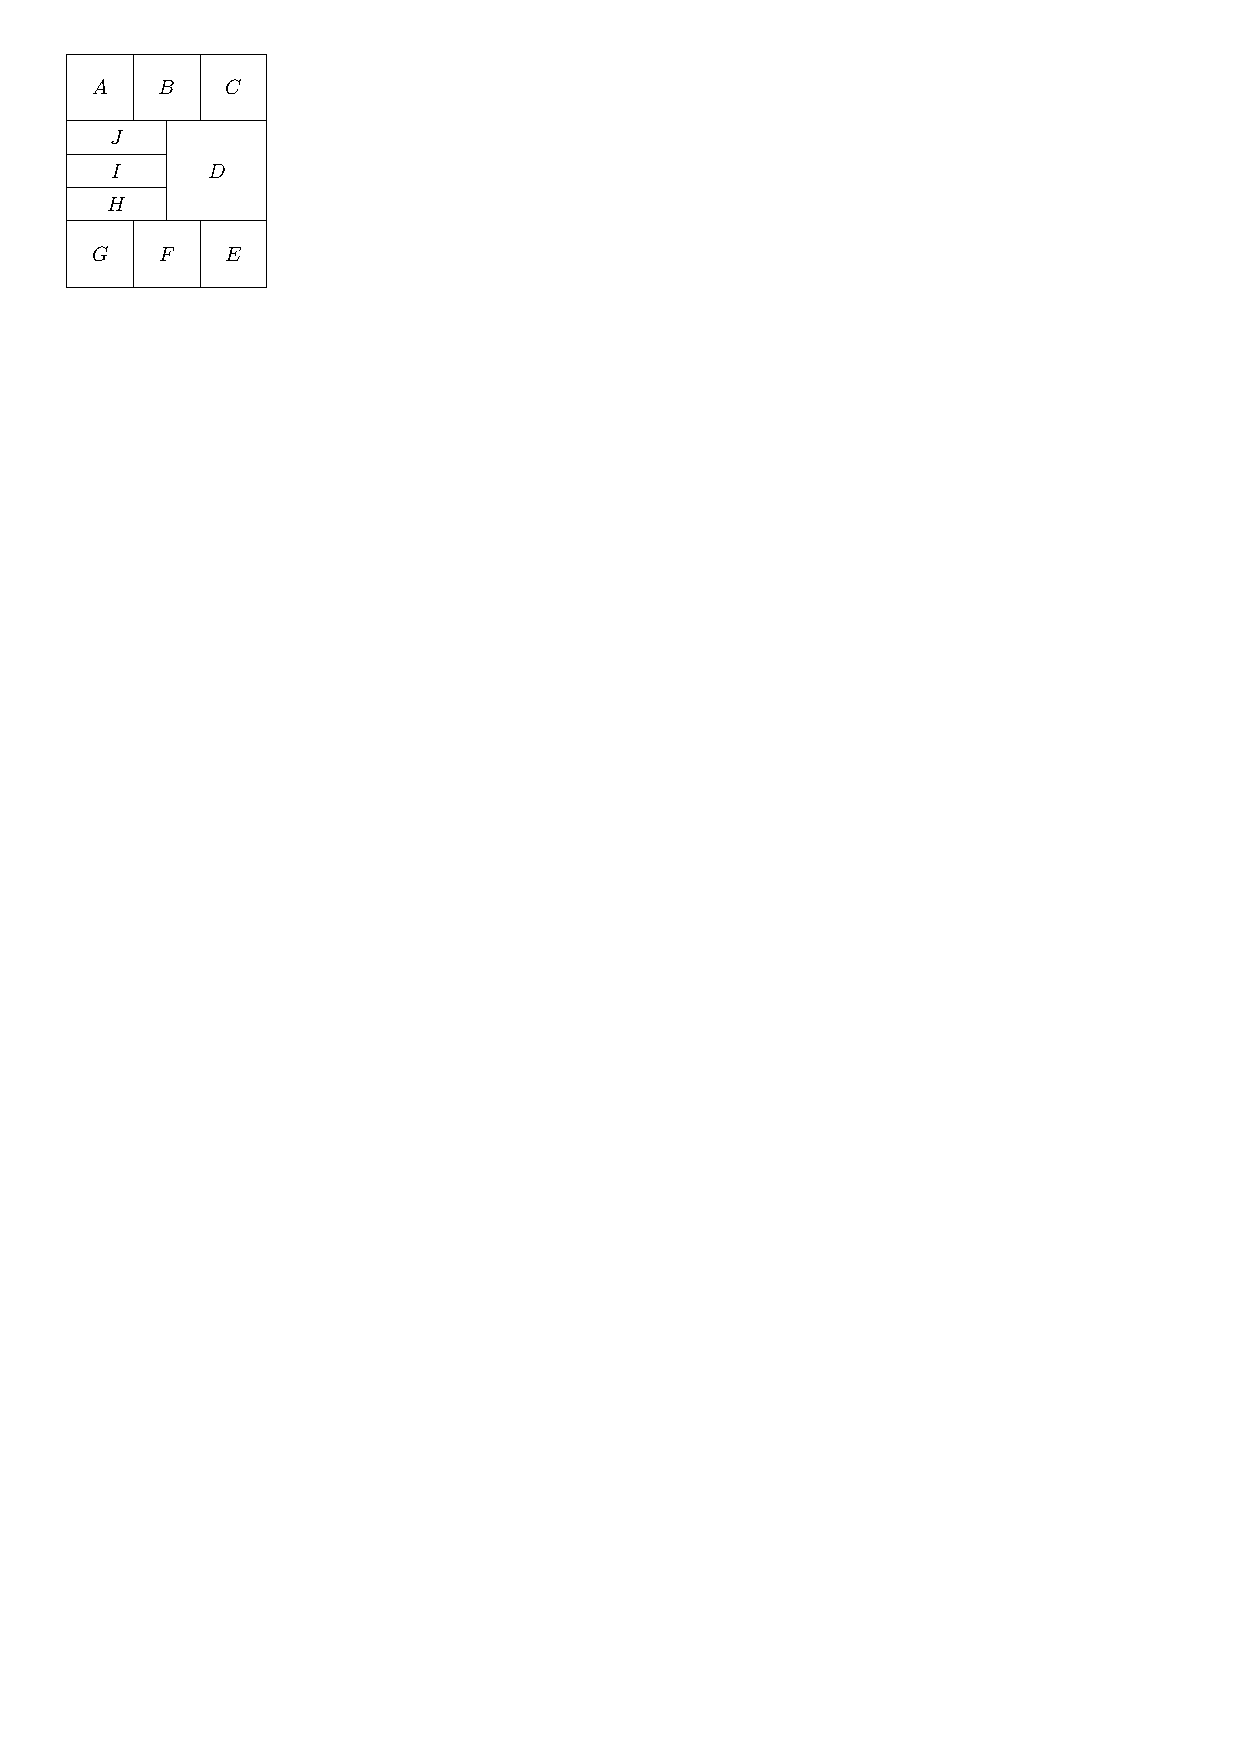
\includegraphics[]{introduction/img/rinsma2Sided.pdf}
    \caption{A 2-sided dual of the Rinsma graph in Figure~\ref{fig:intro:rinsma}.}
    \label{fig:intro:rinsma2Sided}
  \end{wrapfigure}

  That being said, during our research we did not find any graphs without separating $4$-cycles that did not admit any $2$-sided layouts.
  For example, the graph, by Rinsma, without an one-sided dual does have a $2$-sided dual, as can been seen in Figure~\ref{fig:intro:rinsma2Sided}.
  We thus conjecture that these graphs admit a $2$-sided layout and it is just the algorithm for finding them that eludes us.

  Its worthy of note, that the bound obtained by the algorithm is not stronger then the bound provided by the counterexample. That is, there might be an algorithm providing $O(d)$-sided layouts for all graphs $G$ admitting a rectangular dual.

\mypar{Overview}
  The rest of this thesis is focused on obtaining these two results.
  In order to do this we give extensive definitions on graphs, paths and cycles in Section~\ref{s:prelim}. In Section~\ref{s:rel} we introduce the notion of regular edge labellings.  A regular edge labeling is a way of coloring and orienting the edges of a graph that corresponds to a rectangular dual of that graph.
  We frequently use this notion in the rest of this thesis.
  Once we have these preliminaries out of the way, we prove Theorem \ref{fix:th:family} in Section~\ref{s:fix} and Theorem \ref{th:dsided} in Section~\ref{s:algo}. We prove Theorem \ref{fix:th:family} by counterexample and Theorem \ref{th:dsided} by giving a constructive algorithm.
